\chapter{Resultados e discussão}
\label{cap:resultados}

\begin{enumerate}
	
	\item Parágrafo de introdução do capítulo. Citar que, basicmente, o leitor encontrará no capítulo:
		\begin{enumerate}
			\item Resultados do ONEMAX, legitimando o uso do código para o programa mais complexo que foi utilizado no método dos indianos.
			\item o estudo dos tipos de \textit{fitness}, operador responsável pelo elo entre o algoritmo e o problema \cite{Linden2008}, que, para o nosso caso, é encontrar autovalores. Ponte para o próximo: para cada tipo de \textit{fitness}, um resultado diferente.
		\end{enumerate}

	\item Os dois tipos de fitness dos indianos. Ideia central: dois tipos, resultados diferentes. Com $\nabla \rho$ chegamos a um autovalor qualquer, com $(\rho - \rho_0)^2$ podemos chegar ao mínimo, mas dá mais trabalho. Ponte para o próximo: proposta de dois novos fitness.
	
	\item Combinação de $\nabla \rho$ com $(\rho - \rho_0)^2$. Se cada forma leva a comportamentos diferentes, tentamos combinar os dois termos em um único fitness. Uma hipótese seria a melhoria da qualidade dos resultados. A hipótese não foi confirmada. Ponte para o próximo: a busca pela qualidade levou à verificação da importância do parâmetro $\lambda$.
	
	\item Além do que os indianos disseram, que $\lambda$ é escolhido para não estourar a função exponencial, ele tem influência na convergência do algoritmo e na precisão (ou resolução) do fitness. Se na primeira população, geração inicial, o fitness médio é alto, isso provoca convergência precoce, fazendo com que o resultado final seja ruim. Por outro lado, se no início o fitness médio é muito baixo, não há muita discriminação entre os indivíduos, o fitness não cresce e não chegamos a uma solução. A medida que o fitness se aproxima de 1, a discriminação entre os indivíduos fica difícil, levando ao problema da resolução. Ponte para o próximo: vários testes levaram ao desenvolvimento de uma equação empírica para $\lambda$, restrita às matrizes de Coope$-$Sabo \cite{Coope1977}.
	
	\item Fórmula empírica. Por já conhecermos de antemão os autovalores das matrizes de Coope$-$Sabo, foi possível criar uma fórmula empírica para $\lambda$. Ela garante que na primeira população o \textsl{fitness} médio é baixo, previnindo o \textsl{underflow} do \textit{fitness} e a convergência prematura.
	
\end{enumerate}
	
\section{O método não leva ao mínimo global}	

	Retomar brevemente o artigo de 2004. 
	
	Focar no fitness.
	
	Apresentar os parâmetros utilizados no artigo de 2004 \cite{metodo2004} para os testes.
	
	Parâmetros:
	
	\begin{itemize}
		\item Número de indivíduos: 20.
		\item Probabilidade de \textit{crossover}: 0,75.
		\item Probabilidade de mutação: 0,5.
		\item Intensidade de mutação: não fala explicitamente. utilizado 0,01, valor estipulado durante a explicação do método.
		
	\end{itemize}
	
	Aplicação desse parâmetros em matrizes de Coope-Sabo de ordem	N = 10, 20, 30, 40, 50, 60, 70, 80, 90 e 100.
	
	Dez execuções com sementes distintas. (precisão boa)
	
	Gráficos do comportamento do \textit{fitness} (fitness em função das gerações).
	
	Gráficos do comportamento do $\rho$.
	
	Tabela com valores na parada da(o): geração, $\rho$, \textit{fitness}, autovalor relacionado ao mínimo local, erro em relação a esse mínimo local, autovalor que o programa acabou preso (mínimo local).
	
	\textbf{\textcolor[rgb]{1,0,0}{Novidade}}: Verificação empírica que o fitness na forma $f_i = e^{-\lambda(\nabla\rho)^2}$ não leva ao autovalor mínimo, mas está sujeito a mínimos locais.
	
	Explicar retomando os fatos sobre cociente de Rayleigh apresentados no (futuro) capítulo de álgebra linear.
	
	Apesar de não chegar ao mínimo, pode ser utilizado de maneira exploratória. Relembrar as dez execuções anteriores e verificar que houve diferentes autovalores encontrados.
	
	Problema: lentidão. Ponte para ...
	
	\section{$f_i = e^{[-\lambda \nabla \rho]}$ é mais rápido do que $f_i = e^{[-\lambda (\nabla \rho)^2]}$}
	
	Como um dos critérios de parada utiliza $\nabla \rho$ (sem quadrado), testamos essa forma no fitness.
	
	Várias execuções.
	
	Gráfico comparando o comportamento (um termina mais rápido)
	
	Tabela com os detalhes explícitos do do ganho.
	
	Ponte pra falar sobre o outro fitness que encontra o mínimo.
	
	\section{$f_i = e^{-\lambda(\rho_i - \rho_0)^2}$ leva ao autovalor mínimo ($E_0$), mas devemos saber aproximadamente onde ele está}
	
	Justificar esse outro fitness com o artigo de 2006.
	
	Discutir a introdução do novo parâmetro $\rho_0$.
	
	Com $\rho = 0$, realizar exatamente as mesmas execuções da seção anterior.
	
	Realizar dez execuções com precisão boa para N = 10 e N = 100;
	
	Verificar que foi possível chegar no mínimo autovalor.
	
	Exemplos de execução:
	
	
	\begin{enumerate}
		\item \textbf{O que acontece quando $\rho_0$ está um pouco acima de $E_0$?}
		
				Para com $<\rho> \approx \rho_0$
				
				Não encontra o menor autovalor ($E_0$).
				
				Porém, verifica-se que o $<\nabla \rho> \approx 0$.
				
				Então, estamos próximos ao menor autovalor.

				
		\item \textbf{O que acontece quando $\rho_0$ está um pouco abaixo de $\lambda_0$}
						
				Encontra uma aproximação para o autovalor mínimo ($\lambda_0$).
				
				$<fitness>$ é próximo a 1 pois $<\rho>$ é próximo de $\rho_0$.
				
				$<\nabla \rho> \approx 0$.
				
						
		\item \textbf{O que acontece quando $\rho_0$ está muito acima de $E_0$?}
		
					Acredito que não encontrará uma aproximação para $E_0$, pois a região de busca está muito distante. (verificar)
					
				Para com $<\rho> \approx \rho_0$
				
				Verifica-se que o $\nabla \rho >> 0$. Portanto, estamos distantes do menor autovalor.
						
		\item \textbf{O que acontece quando $\rho_0$ está muito abaixo de $E_0$?}
				
				Acredito que não encontrará uma aproximação para $E_0$, pois a região de busca está muito distante.
				
				Para com $<\rho> \approx \rho_0$
				
				Verifica-se que o $\nabla \rho >> 0$. Portanto, estamos distantes do menor autovalor.
		
	\end{enumerate}
	
	Citar brevemente a relação entre a dificuldade (parece uma inércia) de melhorar a precisão dos resultados no final, dizer que isso está relacionado com o formato da função \textit{fitness}.
	
	Ponte para a discussão do \textit{fitness}
	
\section{$f_i = e^{-\lambda(\rho_i - \rho_0)^2}$ próximo de $\rho$ é intrinsicamente impreciso}
	
	Como $\lambda$ e $\rho_0$ são constantes por definição, $f_i$ é uma função apenas de $\rho$.
	
	Função simétrica em torno de $\rho_0$.
	
	Gráfico com diferentes $\rho_0$'s para o domínio $\rho = [-200,200]$. 
	
	Para uma dada função $fitness$, em torno de zero, por exemplo, dar um \textit{zoom} no pico.
	
	\begin{figure}[htbp]
		\centering
			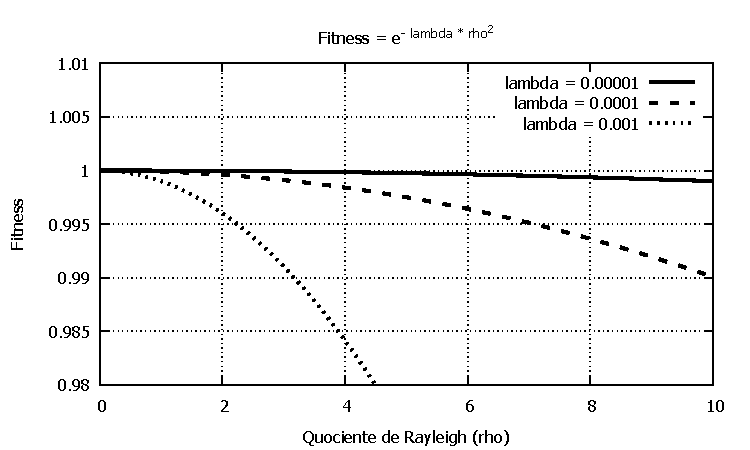
\includegraphics{figs/varios-fit-mono-zoom.pdf}
		\caption{Zoom próximo do pico}
		\label{fig:varios-fit-mono-zoom}
	\end{figure}
	
	
	Gráficos com $\rho = [-5,5]$ e $\rho = [-0.1,+0.1]$.
	
	Verificar que no último gráfico o SciLab já apresenta dificuldades para diferenciar os pontos de $f$.
	
	Gráfico da variação do fitness como função da variação do $\rho$ (a derivada).
	
	A derivada é 
	
	$$
		\frac{df}{d\rho} = -2\lambda(\rho - \rho0)e^{-\lambda(\rho - \rho0)^2}
	$$
	
	Com $\rho = [-200,200]$, gráfico da derivada.
	
	Gráfico comparando $f$ com $df/d\rho$. Verificar visualmente que $df/d\rho$ é muito pequeno, próximo de zero. 
	
	Tabela com os valores mostrando que, próximo à $\rho_0$, uma mudança de $\Delta\rho = 0.1$ leva a uma variação de $\Delta f <= 0.000001$.
	
	Para o algoritmo genético isso é ruim. Cada rho está associado a um indivíduo e o fitness deve diferenciar cada um, de modo que a maior nota é dada ao indivíduo mais próximo da solução.
	
	Veja que para $\rho = [-0.3,+0.3]$ o fitness é igual a 1. Nessa região a o fitness falha na diferenciação dos indivíduos.
	
	Para fitness muito pequeno há o mesmo problema. Com isso, pode-se definir uma região do fitness onde a função é apropriada para o uso dos algoritmos genéticos. Figura \ref{fig:fitness_boaRegiao}.
	
	Para Futuro, continuação do trabalho: há alguma maneira de lidar com os parâmetros de $f$ de modo a ficarmos sempre na região boa?
	
	Região boa: entre as duas linhas, quase linear.
		
	\begin{figure}[htbp]
		\centering
			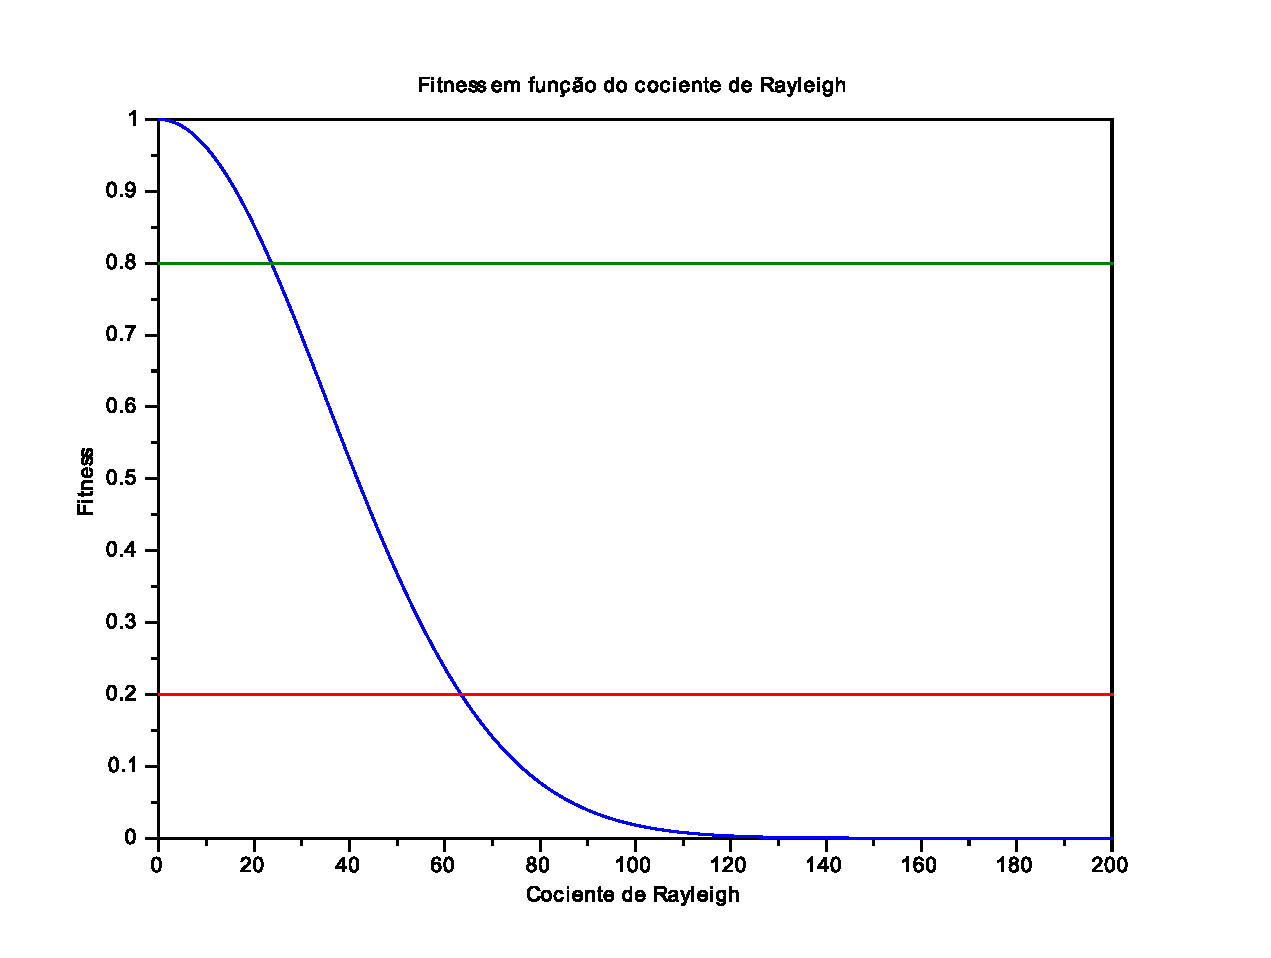
\includegraphics[width=0.90\textwidth]{figs/resultados/fitness_boaRegiao.pdf}
		\caption{Boa região para o fitness (entre as duas linhas)}
		\label{fig:fitness_boaRegiao}
	\end{figure}
	
	Há um limite de precisão intrínseco com o uso desse fitness.
	
	Por isso a dificuldade em melhorar a precisão.
	
	% Table generated by Excel2LaTeX from sheet 'Plan2'
\begin{tabular}{rr}

       \textit{rho} &          \textit{f} \\

      -0,1 &   0,999996 \\

     -0,09 &   0,999997 \\

     -0,08 &   0,999997 \\

     -0,07 &   0,999998 \\

     -0,06 &   0,999999 \\

     -0,05 &   0,999999 \\

     -0,04 &   0,999999 \\

     -0,03 &          1 \\

     -0,02 &          1 \\

     -0,01 &          1 \\

         0 &          1 \\

      0,01 &          1 \\

      0,02 &          1 \\

      0,03 &          1 \\

      0,04 &   0,999999 \\

      0,05 &   0,999999 \\

      0,06 &   0,999999 \\

      0,07 &   0,999998 \\

      0,08 &   0,999997 \\

      0,09 &   0,999997 \\

       0,1 &   0,999996 \\

\end{tabular}  

		
		O parâmetro $\lambda$ também influencia fortemente o fitness e o algoritmo genético.
		
		Ponte para a discussão do $\lambda$.
		
	\section{Por que o $\lambda$ deve ser escolhido cuidadosamente?}
	
	Execuções para N=10 com diferentes $\lambda$'s. Com os gráficos, explicar o que o artigo de 2004 quis dizer com \textit{fitness overflow/underflow}.
	
	Gráficos com rho entre 0 e 250 (exemplo pra N=10), mas com cortes em diferentes rhos.
	
	\begin{figure}[pt]
	\centering
		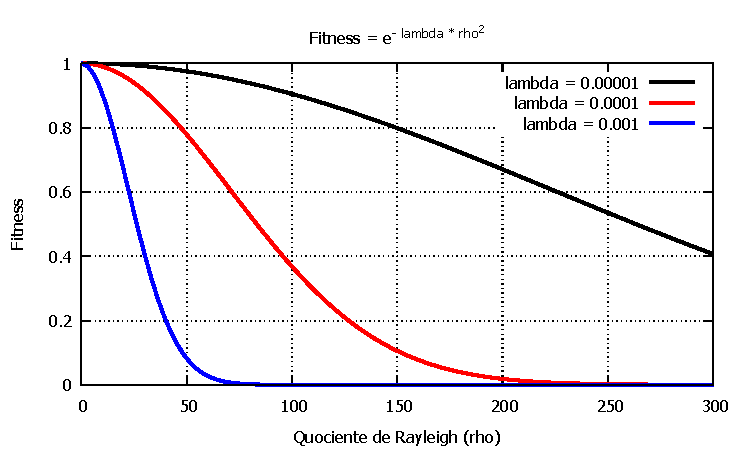
\includegraphics{figs/varios-fits-color.pdf}
	\caption{Fitness em função do lambda $-$ colorido}
	\label{fig:varios-fits-color}
\end{figure}

\begin{figure}[pb]
	\centering
		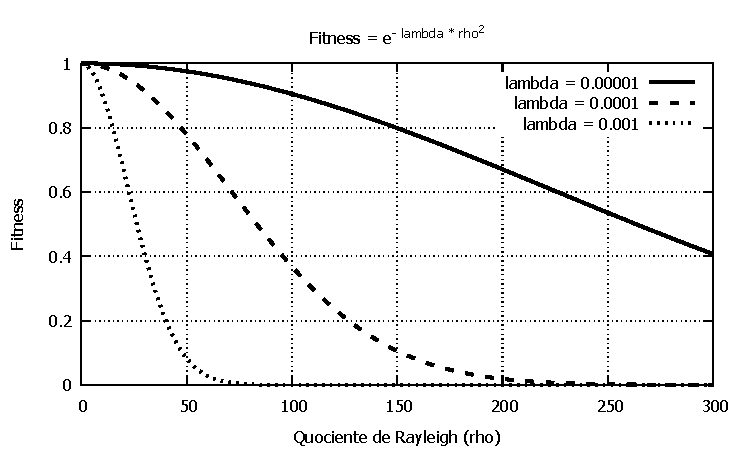
\includegraphics{figs/varios-fits-mono.pdf}
	\caption{Fitness em função do lambda}
	\label{fig:varios-fits-mono}
\end{figure}

	Explicar que uma boa escolha do $\lambda$ deve cobrir todos os autovalores. Citar as execuções anteriores (boas e ruins em função de cada $\lambda$).
	
	Gráfico com $\lambda$ fazendo o fitness cortar em um $\rho$ muito baixo. Discutir puxando as execuções anteriores.
	
	Outro gráfico, mas com $\lambda$ fazendo o fitness cortar em um $\rho$ muito alto. Discutir puxando as execuções anteriores.
	
	Gráfico com uma boa escolha de $\lambda$. Discutir puxando as execuções anteriores.
	
	Após estimativa, refinar a obtenção do $\lambda$. Alterar o $lambda$ (valores em torno da estimativa), executar o programa para verificar se o fitness médio da primeira população é baixo. (se a população inicial tem fitness muito grande, há convergência prematura).
	
	Tabela com alguns $lambdas$ encontrados dessa maneira (estimativa e refinamento).
	
	Infelizmente, para cada matriz, um $\lambda$ diferente.
	
	Ponte pra equação empírica do $\lambda$.
	
	\section{Equação empírica para o $\lambda$}
	
	Delineamento da equação como feito na reunião de 29/09.
	
	Isolar $\lambda$ a partir da $f=e^{-\lambda*(\rho - \rho_0)^2}$
	
	Fazer $f = 0.00001 \approx 0$.
	
	Substituir $(\rho - \rho_0)^2$ por $E_{central} - E_{mínimo}$. Justificar.
	
	Regressão linear para $E_{central} - E_{mínimo}$ com função apenas da ordem da matriz (N).
	
	Inserir a Equação obtida na regressão na equação de $\lambda$.
	
	Fator $0.65$: obtido empiricamente de modo que o $\lambda$ seja semelhante aos encontrados pelo processo de estimativa e refinamento.
	
	Exemplo de execução com $\lambda$ automático.
	
	Explicitar que essa equação é válida apenas para matrizes de Coope-Sabo. Apesar disso, foi importante para o estudo pois permitiu automação completa.
		
	\section{A mistura de $(\rho - \rho_0)^2$ com $\nabla\rho$ não leva a melhores resultados}
	
	Como em seção anterior verificamos que $f_i = e^{[-\lambda \nabla \rho]}$ é mais rápido do que $f_i = e^{[-\lambda (\nabla \rho)]}$, e que o $\nabla\rho$ está diretamente associado aos autovalores, pensei na seguinte hipótese: inserir $\nabla \rho$ ao fitness com $(\rho - \rho_0)^2$ traria resultados mais rápidos.
	
	Justificativas para a hipótese: 
	
	\begin{enumerate}
		\item Inserir $\nabla \rho$ no fitness puniria os $\rho$'s que, apesar de próximos de $\rho_0$, não fossem autovalor. Em outras palavras, o termo $\rho - \rho_0 \approx 0$, mas $\nabla \rho >> 0$ e, portanto, o fitness ficaria pequeno.
		
		\item Como o fitness, a princípio, estaria diferenciamento melhor os bons indivíduos, o algoritmo teria uma taxa de convergência maior.
		
	\end{enumerate}
	
		Executar $10$ para o primeiro fitness, e, utilizando as mesmas dez sementes, executar outros $10$ testes com ou outro fitness.
		
		Comparação dos resultados: gráficos do comportamento do fitness e tabela comparando a velocidade de convergência (em que geração o critério de parada foi atingido), tempo de execução e erro relativo ao menor autovalor ``exato'' (obtido no SciLab).
	
	\section{Resultados preliminares na GPU}
	
		\subsection{ONEMAX na GPU}
	
				ERAD: artigo $+$ poster
				
		\subsection{Método paralelizado (versão atual, com ganho de $1,4$}
		
				Falar um pouco.
		
				